\documentclass[output=paper,newtxmath,modfonts,nonflat,draftmode]{langsci/langscibook} 
\ChapterDOI{10.5281/zenodo.3520567}

\title{Variable word-final vowel deletion and reduction in Gurmancema: A maximum entropy model} 
\author{Maggie Baird\affiliation{Dartmouth College}}

\abstract{Gurmancema (Gur, Burkina Faso) displays an overall dispreference for word-final tense vowels phrase-medially. On the surface, there is vowel reduction and vowel deletion, which vary both across and within phonological contexts. This work will provide an overview of the complex data patterns and describe a weighted constraint approach to the data patterns using a Maximum Entropy Harmonic Grammar. Weighted constraints are preferred to ranked constraints due to variability in the data and to account for cases of constraint ganging, including superadditivity.}

\begin{document} 
\shorttitlerunninghead{Variable word-final vowel deletion and reduction in Gurmancema}

\maketitle
\section{Introduction}\label{sec:baird:1}
Gurmancema (ISO 639-3: gux), also known as Gulmancema, Gourmanchema, or Gourmanché, is a Gur language spoken in Burkina Faso, Togo, Benin, and Niger. It has approximately 1 million speakers across this region \citep{ethnologue}. Primarily a spoken language, there is much dialectal variation across speakers in different villages and areas. Gurmancema is an SVO language with three tones (H, M, L). 

Gurmancema has a five vowel system /a, e, i, o, u/. In this paper, I take these five phonemic vowels to be [+tense] and the allophone [ə] to be [\textminus tense].\footnote{The feature [tense] is used for convenience to distinguish peripheral vowels from the central vowel [ə] and is not meant to make theoretical claims about the [tense] status of these vowels. The markedness constraints \textsc{Ident}[tense] has a weight of 0 in the model and does not change the analysis.}  /aː, iː, uː/ are phonemic in Gurmancema and contrast with /a, i, u/. There are conflicting accounts of whether the long vowels /eː, oː/ are also phonemic.\footnote{For grammars containing phoneme inventories and justifications, see \citet{Chantoux1968} and \citet{Naba1994}.} There is also debate over which diphthongs are phonemic in the language. My analysis only makes reference to short, word-final monophthongs, so I remain agnostic.

\tabref{tab:baird:1} shows the consonant inventory of Gurmancema for the dialect of study in this paper. See \sectref{sec:baird:4} for more information about the dialect in question.

\begin{table}
\caption{Consonant Inventory of Gurmancema}
\label{tab:baird:1}
\begin{tabularx}{\textwidth}{Xcccccc}
\lsptoprule
  & Labial & Alveolar & Palatal & Velar & Labiolvelar & Glottal\\ 
 \midrule
 Stop & p, b & t, d & c, ɟ & k, g & k͡p, g͡b & \\
 Fricative & f & s &  &  &  & h\\
 Nasal & m & n & ɲ & ŋ & ŋ͡m & \\
 Liquid &  & l &  &  & & \\
 Tap &  & ɾ  &  &  &  & \\
 Glide & w & & j & &  & \\
 \lspbottomrule
 \end{tabularx}
\end{table}


\sectref{sec:baird:2} of this paper describes the complex data patterns in question in this study. In \sectref{sec:baird:3}, I will discuss previous work in Gurmancema and on similar patterns 
of vowel deletion. \sectref{sec:baird:4} describes the data collection and analysis process. \sectref{sec:baird:5} presents a constraint-based analysis of a few illustrative phonological environments. In \sectref{sec:baird:6}, I will summarize my findings. 

\section{Data presentation} \label{data}\label{sec:baird:2}
In Gurmancema, word-final vowels in verbs and nouns are often deleted or reduced to [ə] in phrase-medial position. The surface representation of these vowels depends on many factors, including the sound that follows them. For example, in cases of vowel hiatus, the word-final vowel of the first word is always deleted, shown in (\ref{vowels}):

\ea \label{vowels}
\gll /súnd-i à=bób=à/ \hspace{0.5cm} [súnd àbóbà]\\
forget-\textsc{asp} \textsc{cl.pl}=jug=\textsc{cl.pl}\\
\glt `forgets jugs'
\z

The behavior of the word-final vowel also depends on the sound that precedes it. For example, the vowels /a, i, o/ all reduce to [ə] when preceded by an obstruent, shown in (\ref{obs}):
  
\ea \label{obs}
\ea \gll /kì=bé=ga pwá/  \hspace{0.5cm} [kìbégə pwá] \\
 \textsc{cl.sg}=child=\textsc{cl.sg} hit\\
\glt `child hits'

\ex 
\gll /ti=k͡pén=dì pwá/ \hspace{0.5cm} [tik͡ṕendə̀ pwá]\\
\textsc{cl.sg}=sauce=\textsc{cl.sg} hit\\
\glt `sauce hits'

\ex
\gll /o=ŋumb=o pwá/ \hspace{0.4cm} [oŋumbə pwá]\\
\textsc{cl.sg}=donkey=\textsc{cl.sg} hit\\
\glt `donkey hits'
\z 
\z

As can be seen, many factors come together to influence the surface representation of underlying vowels, not just what sound precedes or follows the vowel. Different vowels behave differently in the same context. /i/ reduces to [ə] when preceded by an approximant (\ref{ex:baird:approx:a}), but /a/ will surface as [a] in the same immediate phonological environment (\ref{ex:baird:approx:b}). 

\ea \label{ex:baird:approx}
\ea \label{ex:baird:approx:a}
\gll /da=lì pwá/ \hspace{0.8cm} [dalə̀ pwá]\\
friend=\textsc{cl.sg} hit\\
\glt `friend hits'

\ex \label{ex:baird:approx:b}
\gll /a=bé=la pwá/ \hspace{0.5cm} [abéla pwá]\\
\textsc{cl.pl}=child=\textsc{cl.pl} hit\\
\glt `children hit'
\z
\z

To complicate matters, certain patterns in Gurmancema are categorical, while others are variable. In (\ref{obs}), I showed that /a, i, o/ categorically reduce to [ə] when preceded by obstruents, but the vowel /u/ shows a variable pattern. The percentages and token counts are from the sample included in this paper, which consists of data elicited from one speaker. 

\ea \label{u}
\ea
\gll /bú=tí=bu k͡pá/  \hspace{0.6cm} [bútíbu k͡pá] (67\%, $n=3$) \\
 \textsc{cl.sg}=tree=\textsc{cl.sg} kill \hspace{0.5cm} [bútíbə k͡pá] (33\%, $n=3$)\\ 
\glt `tree kills'

\ex
\gll /kú=dá=gu k͡pá/  \hspace{0.5cm} [kúdágu k͡pá] (67\%, $n=3$) \\
 \textsc{cl.sg}=wood=\textsc{cl.sg} kill \hspace{0.5cm} [kúdágə k͡pá] (33\%, $n=3$)\\ 
\glt `wood kills'
\z
\z

As these examples show, this is a case of token variation, where the same word can be pronounced differently on different occasions with no change in meaning. 

Word-final vowels preceded by the bilabial nasal also show a variable pattern, which is not only predictable by the CV combination, but also takes into account the first consonant of the next word. When the next word begins with a bilabial consonant, the vowel varies between reduction and deletion, but when the consonant has a different place of articulation, the vowel is much more likely to reduce. 

\ea \label{m}
\ea
\gll /mí=ɟe=má pwá/ \hspace{0.5cm} [míɟem pwá] (67\%, $n=6$)\\
 \textsc{cl.sg}=food=\textsc{cl.sg} hit  \hspace{0.5cm} [míɟemə́ pwá] (33\%, $n=6$)\\ 
\glt `food hits'

\ex
\gll /mí=ɟe=má k͡pá/ \hspace{.5cm} [míɟemə́ k͡pá] (88\%, $n=32$)\\
\textsc{cl.sg}=food=\textsc{cl.sg} kill \hspace{0.5cm} [míɟem k͡pá] (12\%, $n=32$)\\
\glt `food kills'
\z
\z

(\ref{sum}) lays out the general data patterns presented above:

\ea \label{sum}

V + \# + V \hfill deletion of the first vowel \newline
Obstruent + /a, i, o/ + \# + C \hfill reduction of the vowel\newline
Obstruent + /u/ + \# + C \hfill variation between reduction and deletion\newline
Non-nasal sonorant + /i/ + \# + C \hfill reduction of the vowel\newline
Non-nasal sonorant + /a/ + \# + C \hfill no reduction or deletion\newline
/m/ + /a, i, o/ + \# + Non-Bilabial C \hfill reduction of the vowel\newline
/m/ + /a, i, o/ + \# + Bilabial C \hfill variation between deletion and reduction\newline

\z

There are several environments which are not included in this analysis. /e/-final words are morphologically distinct and involve a different set of constraints than is presented below. Other environments, such as non-nasal sonorant + /o, u/, and /m/ + /u/ are missing due to a lack of data. 

In this paper, I will walk through a constraint-based analysis that models all of these patterns and also accounts for the variation. Vowel reduction and deletion have been noted in the literature on Gurmancema, but never fully analyzed including variation. The model incorporates 13 constraints and necessitates supperadditivity \citep{AlbrightMagri2008,GreenDavis2014} to account for the patterns in the most economical way. 



\section{Previous work} \label{sec:baird:3}

In the literature on Gurmancema, there is not a complete account of vowel deletion and variation. \citet{Naba1994} notes that three authors have touched on issues of reduced vowels from a phonotactic perspective, but they all have different analyses. He says that too little attention has been paid to elision, apocope, and assimilation and that the description and analysis of these phenomena are very important for tonal and morphological reasons.

The only work focusing specifically on vowel deletion and reduction is \citet{Rialland1980,Rialland2001}. She labels the process “vowel punctuation and deletion'', arguing that there are weak and strong forms of words.  Strong forms occur at the ends of phrases, where word-final vowels are maintained. In weak position, or phrase-medially, she argues that vowels are deleted and an epenthetic [i] is inserted to prevent illicit consonant clusters. She argues that these processes do not affect monosyllabic words. In \citet{Rialland2001}, she elaborates that monosyllabic words are slightly lengthened. Her paper does not attempt a constraint-based analysis -- I will argue that these frameworks are better suited to representing the data than rule-based phonology. 
	
Across Niger-Congo languages, vowel elision is also common as a repair for vowel hiatus. Across word boundaries, the first vowel is always deleted \citep{Casali1997}, which holds true for Gurmancema. Although this is one aspect of the vowel-deletion process in Gurmancema, vowels do not only delete in hiatus contexts in Gurmancema, as can be seen in the examples in (\ref{m}). There is no process analagous to the word-final vowel reduction in Gurmancema that I could find in the Niger-Congo literature. 
 
\section{Data collection and analysis}\label{sec:baird:4}

All of the data in this paper are based on the speech of a 37-year-old female speaker from the village of Mahadaga, currently living in France. All data were elicited in summer 2016. I designed an elicitation plan with the aim of obtaining every possible CV\#C combination in the language across Subject-Verb and Verb-Object boundaries. I also elicited data in other syntactic conditions, such as relative clauses and Adjective-Noun pairings, but this paper will focus solely on the Subject-Verb and Verb-Object interfaces. There were restrictions on phonemic distribution, however, as Gurmancema has multiple noun classes, marked by proclitics and enclitics.  Nouns only begin and end with certain sounds, with a few exceptions. I created an elicitation plan that included 26 nouns used as subjects, with 25 different CV endings. I elicited 20 transitive verbs and 4 intransitive verbs with each of the subjects. Verbs had to vary with both the initial consonant and the final CV, and I attempted to include as many environments as possible at both edges. 

This study aims to provide a phonological analysis grounded in acoustic phonetics rather than perception. The informing data were not field notes, but rather the database of acoustic measurements. I tagged every word-final vowel ($n=3855$) in my Gurmancema sample for important values: the vowel (a, e, i, o, u), the preceding phoneme, the following phoneme, the role in the sentence (S, V, O), the surface form (maintained, reduced, deleted), whether it was followed by a pause, the length of the vowel in seconds (3 decimal points), and F1, F2, and 
F3. All phonetic measurements were made in Praat \citep{Boersma1996} by hand. Given the large number of attributes I was tracking, I did not find a script that I thought would be more efficient than taking measurements by hand. I took formant measurements at the middle of the vowel in the most stable portion of the formants. There is a possibility for human error and measurement variation, but taking formant measurements by hand allowed me to evaluate any problematic data points individually. Formant measurements were taken for a total of 3855 vowels, including diphthongs ($n=200$) and phrase-final vowels ($n=1297$), which were not included in the final 
analysis. Phrase-final vowels were not included as the reduction and deletion processes do not apply at the end of phrases. I also did not analyze any pre-pausal data from slow speech. The goal of this study was to model naturalistic speech and not have any confounding effects from pauses. 

I used formant measurements to determine whether a vowel was maintained or reduced. I took a sample of canonically maintained vowels and took mutually exclusive ranges in F1 and F2 to determine whether the more ambiguous cases were maintained or reduced. The results of my phonetic analysis show that there is one central reduced vowel [ə], which can be seen in Figure 1. Although schwa does seem to overlap with the vowels /o/ and /u/, none of the cases where [ə] is that far back and high are underlyingly /o/ and /u/. These are cases of reduced /i/ and /a/.



\begin{figure} 
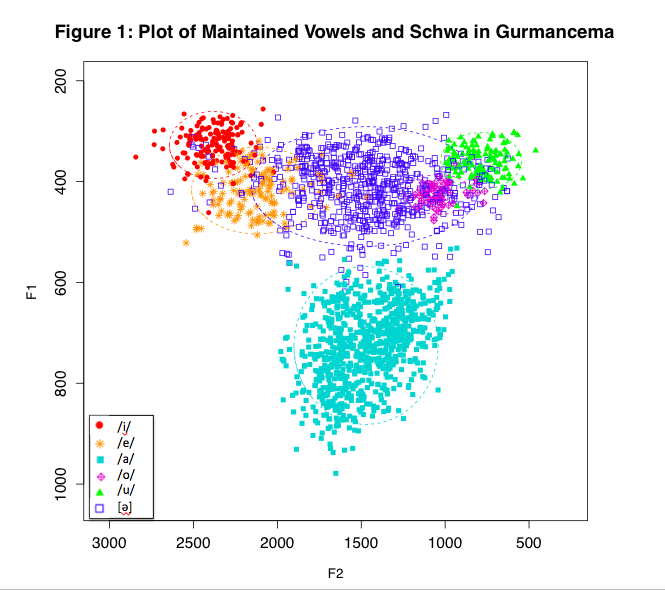
\includegraphics[width=10cm]{figures/ACAL_Vowel_plot.png} % width calculated from image resolution @ 300 dpi.
\caption{Plot of maintained vowels and schwa in Gurmancema. Note: Ellipses mark standard deviations from the mean formant values of each vowel.}
\end{figure}
 

Throughout the analysis, the term “prevocalic consonant” refers to the consonant that is in penultimate position of the given word (i.e. the onset of the final syllable). The term “following consonant” refers to the first consonant of the following word. 

For example, in the phrase /kìbéga pwá/ `child hits', the prevocalic consonant is /g/ and the following consonant is `p'. 

In general, there are three surface forms for vowels. If a vowel surfaces the same in the output and the input, I will refer to it as ``maintained.'' If a vowel surfaces as [ə], I will refer to it as ``reduced.'' If a vowel is deleted, I refer to it as ``deleted.''

\section{Constraint-based analysis}\label{sec:baird:5}
In this section, I will explain the model I used to analyze the data. 

\subsection{Maximum Entropy Harmonic Grammar}\largerpage

Due to the complex and variable nature of the process, these data are well-suited to a constraint-based analysis. A major component of the complexity in the Gurmancema data is the free variation, which necessitates a stochastic constraint-based model. In this paper, I use Maximum Entropy Harmonic Grammar (MaxEnt), which captures patterns of variation \citep{GoldwaterJohnson2003,HayesWilson2008}. 
	 
In MaxEnt, each candidate receives as score, which is calculated the same way as Harmony in traditional Harmonic Grammar (HG), by summing the weights of violations incurred. The calculation of the score h(\textit{x}) is as follows: 

\ea
$ \mathrm{h}(x) = \sum_{\textit{i}=1}^{\textit{N}}$ ${w_i}{C_i}(x)$
\z

${w_i}$ is the weight of the $i$th constraint, ${C_i}(x)$ is the number of times $x$ violates the $i$th constraint, and the sum is the summation over all constraints in the model.  

The MaxEnt grammar tool \citep{WilsonHayesGeorge08} optimizes all of the constraints and assigns each of them weights that can most closely match the observed probabilities of each candidate. Essentially, the probability of any given candidate is calculated from its score in comparison to the scores of all the candidates. For example, if each of two candidates have a score of 1, they will have a probability each of 0.5, so they will each be selected 50\% of the time by speakers as they are equally well-formed.

The probability P(\textit{x}) is calculated as follows based on all the possible forms in Ω:

\ea 
$ \mathrm{P}(x) = \frac{\mathrm{exp}(-\mathrm{h}(x))}{Z}\text{, where } Z = \sum_{y\in \mathrm{Ω}} \mathrm{exp}(-\mathrm{h}(y))$  
\z

The base of the natural logarithm \textit{e} is raised to the negative of the score, and the probability is calculated over all possible forms. 

\subsection{Fitting the model}

I split my data into unique CV\#C combinations, and entered each with its observed probabilities into the learner. The model input consists of a set of constraints, an underlying form, and several (usually 2--6) plausible output candidates, each with observed probability computed from my phonetic analysis. In total, I entered 364 unique tableaux into the MaxEnt Grammar Tool, with standard settings. The model generates weights for each of the constraints that yield the probabilities closest to the observed probabilities. In total, the model required 13 constraints to model the patterns observed in the data. 

\subsection{Initial constraints}
In this section, I will present the initial constraints that are the minimum set to account for the simplest data patterns. As I go through the different patterns in more detail, I will describe and add any other necessary constraints. A full list of constraints and their final weights can be found in \sectref{baird:fulllist}. 

Other models for reduction and deletion often attribute vowel reduction and deletion to prosodic motivators. In Gurmancema, it is the word-final position that is targeted for reduction and deletion regardless of tone or stress (which does not appear to be a salient prosodic feature of the language). For this reason, the constraint I am using to explain this pattern is simply a markedness constraint targeting word-final tense vowels in the language. All data in this paper are phrase-medial, so each constraint is assumed to be phrase-bounded. 

The overall dispreference for word-final tense vowels is captured by the 
mar\-kedness constraint \textsc{NoFinalTenseVowel}:

\ea
\textsc{NoFinalTenseVowel} (*[+tns]\#): Assign a violation for every word-final tense vowel
\z

The repairs triggered to satisfy *[+tns]\#, either by reducing a word-final vowel or deleting it, come with faithfulness violations. By reducing a vowel from any of the phonemic vowels to [ə], the vowel changes the feature [+tense] to [\textminus tense]. This change violates the \textsc{Ident}(tense) constraint, which penalizes changes in the feature [tense] from the input to the output. In the final model, however, this constraint did not ever influence a winning candidate, so it is omitted from the rest of the paper.

Reducing a vowel changes other features, so reduction is penalized through more specific constraints, described in 
(\ref{faithful}).


\ea \label{faithful}
\ea \textsc{Ident-IO(Low)} (\textsc{Ident}(lo)): Assign a violation for every segment that does not surface with the same value for [low] in the input and the output.
\ex \textsc{Ident-IO [Labial]} (\textsc{Ident}(lab)): Assign a violation for every segment that does not surface with the same value for [labial] in the input and output.
\ex \textsc{Ident-IO [High]} (\textsc{Ident}(hi)):  Assign a violation for every segment that does not surface with the same value for [high] in the input and the output. 
\z
\z 

\textsc{Ident}(lo) penalizes /a/ when it raises to [ə], but does not target any other underlying vowels. \textsc{Ident}(hi) penalizes /i/ and /u/ when they lower to [ə], and \textsc{Ident}(lab) penalizes /u/ and /o/ when they reduce. As described in (\ref{data}), these vowels behave differently in the same surrounding contexts, which is why three different \textsc{Ident} constraints are necessary rather than the general \textsc{Ident}(tense) constraint. 
 
The faithfulness that penalizes vowel deletion is \textsc{Max}(V), described below:
  
\ea
\textsc{Maximize(Vowel)} (\textsc{Max(V)}): Assign a violation for every vowel in the input 	that does not surface in the output. 
\z

Constraints that interact with subsets of the data more specifically will be 
presented in the following sections. 

\subsection{Vowel hiatus resolution}

Gurmancema has a vowel hiatus resolution process similar to other Niger-Congo languages \citep{Casali1997}. 
The markedness constraint that motivates the hiatus resolution is as follows:

\ea
 (*V.V): Assign a violation for every sequence of vowels across a syllable boundary. 
\z
  
Vowel hiatus in Gurmancema is always resolved by deleting the first vowel, or the word-final vowel. A tableau showing an example is shown in \tabref{tab:baird:2}.
   
\begin{table}
\caption{Tableau for /di\#a/ with sample phrase ‘forgets jugs’, $n=10$}
\label{tab:baird:2}
\small
{\begin{tabularx}{\textwidth}{Xrrr *{4}{S[table-format=1.2]}} 
\lsptoprule
{} &   \multicolumn{2}{c}{p}  &    &   \multicolumn{1}{c}{*V.V}   &   \multicolumn{1}{c}{*[+tns]\#}   &   \multicolumn{1}{c}{\textsc{Max} (V)}   &   \multicolumn{1}{c}{\textsc{Ident} (hi)}  \\\cmidrule(lr){2-3}\cmidrule(lr){5-8}
/súndi àbóbà/ & obs & pred & score & 9.34 & 6.14 & 3.62 & 2.99 \\
\midrule
{a. [súndi àbóbà]} & 0 & \textasciitilde 0 & 15.44 & 1 & 1 & 0 & 0 \\
{b. [súndə àbóbà]} & 0 & \textasciitilde 0 & 12.63 & 1 & 0 & 0 & 1 \\
{c. [súnd àbóbà]} & 1 & \textasciitilde 1 & 3.62 & 0 & 0 & 1 & 0 \\
 \lspbottomrule\end{tabularx}} 
\end{table}

In the tableau in \tabref{tab:baird:2}, candidate (a) has a vowel sequence and a word-final tense vowel, so it violates *V.V and [+tns]\#, incurring a score of $9.34+6.14$, totaling 15.44. Candidate (b) violates *V.V and \textsc{Ident}(hi), incurring a score of $9.34+2.99$, totaling 12.63. Candidate (c) only violates \textsc{Max}(V), incurring a score of 3.62. This is the lowest score by a significant amount, so the model predicts candidate (c) will surface approximately 100\% of the time, which is what was observed. 
Vowel hiatus resolution is entirely regular and predictable in Gurmancema, with 
the word-final vowel always being deleted.

\subsection{Prevocalic obstruents}
Consonant clusters beginning with obstruents are highly marked in Gurmancema, 
leading to a preference for reduction over deletion when word-final vowels are preceded by an obstruent. In other words, word-final vowels are dispreferred, but when deletion would lead to an illicit consonant cluster, reduction is the preferred fix. The vowels /a, i, o/ reduce when preceded by an obstruent over 90\% of the time. The vowel /e/ is not addressed in this paper, as in the dataset it is always part of root material, which behaves differently from affixal/clitic material. The vowel /u/, however, shows variation when preceded by an obstruent. To start to account for this data, a new constraint is needed, penalizing consonant clusters beginning with obstruents. This is not a general *CC constraint, because not all consonant clusters are equally marked in Gurmancema (see \ref{data}). 

\ea \label{tc}
*[\textminus sonorant][+consonantal] (*TC): Assign a violation for every [\textminus sonorant][+consonantal] consonant cluster in the output. 
\z

\tabref{tab:baird:3} shows an example of reduction of a vowel following an obstruent. The tableau shows observed data for all /Ta\#C/, meaning all environments of an obstruent followed by /a/ followed by a consonant. 

\begin{table}
\caption{Tableau for /Ta\#C/ with sample phrase ‘child loses’, $n=88$}
\label{tab:baird:3}
\small
\begin{tabularx}{\textwidth}{Xrrr *{4}{S[table-format=1.2]}} 
\lsptoprule
{} &  \multicolumn{2}{c}{p}  &    &   \multicolumn{1}{c}{*[+tns]\#}   &   \multicolumn{1}{c}{*TC}   &   \multicolumn{1}{c}{\textsc{Max} (V)}   &   \multicolumn{1}{c}{\textsc{Ident} (lo)} \\\cmidrule(lr){2-3}\cmidrule(lr){5-8}
   /kìbéga bìáni/ & obs & pred & score & 6.14 & 4.55 & 3.62 & 3.52 \\
   \midrule
{a. [kìbéga bìáni]} & 0.05 & \textasciitilde 0.07 & 6.14 & 1 & 0 & 0 & 0 \\
{b. [kìbégə bìáni]} & 0.91 & \textasciitilde 0.92 & 3.52 & 0 & 0 & 0 & 1 \\
{c. [kìbég bìáni]} &  0.04 & \textasciitilde  0.01 & 8.17 & 0 & 1 & 1 & 0 \\
\lspbottomrule\end{tabularx}
\end{table}


Word-final /i/ and /o/ behave very similarly to word-final /a/ when preceded by 
an obstruent, but /u/ behaves slightly differently. Reducing /u/ violates both 
\textsc{Ident}(hi) as well as \textsc{Ident}(round), so the reduced candidate 
has more penalties than the other word-final vowels. This leads to a case of 
ganging, where the violation of two lower constraints is strong enough to overpower one stronger constraint, leading to variation. While violating either \textsc{Ident}(high) or \textsc{Ident}(labial) produces patterns similar to those seen in \tabref{tab:baird:2}, violating both means almost double the penalty for that candidate, making reduction a significantly worse choice for /u/ than the other vowels. The ganging and variation is 
illustrated in \tabref{tab:baird:4}. 

\begin{table}
\caption{Tableau for /Tu\#C/ with sample phrase ‘tree wants’, $n=141$}
\label{tab:baird:4}
\footnotesize
\fittable{%
\begin{tabular}{l l r r *{5}{S[table-format=1.2]}}
\lsptoprule
{} &  \multicolumn{2}{c}{p}   &    &   \multicolumn{1}{c}{*[+tns]\#}   &   \multicolumn{1}{c}{*TC}   &   \multicolumn{1}{c}{\textsc{Max} (V)}   &   \multicolumn{1}{c}{\textsc{ident}(lab)}   &   \multicolumn{1}{c}{\textsc{ident}(hi)}  \\
\cmidrule(lr){2-3}\cmidrule(lr){5-9}
 /bútíbu bwà/ & \multicolumn{1}{c}{obs} & pred & score & 6.14 & 4.55 & 3.62 & 3.62 & 2.99 \\
 \midrule
{a. [bútíbu bwà]} & 0.69 & \textasciitilde 0.57 & 6.14 & 1 & 0 & 0 & 0 & 0\\
{b. [bútíbə bwà]} & 0.31 & \textasciitilde 0.35 & 6.61 & 0 & 0 & 0 & 1 & 1 \\
{c. [bútíb bwà]} & 0 & \textasciitilde    0.08 & 8.17 & 0 & 1 & 1 & 0 & 0\\

\lspbottomrule\end{tabular}}
\end{table}

The model is very accurate in predicting the distribution for maintenance (a) and reduction (b), but the predictions are slightly off, leading to an over-prediction of deletion (c), which was not observed. This is a result of the model being more general. The goal of this analysis was to account for the data with the simplest set of phonological constraints rather than overfitting the model by tailoring constraints to small subsets of data. *TC does not have a higher weight due to the few exceptional cases where TC consonant clusters occur as a result of deletion. \textsc{Max}(V), the only other constraint violated by (c), does not have a higher weight due to cases of vowel deletion elsewhere in the data. 

\subsection{Prevocalic approximants}

Prevocalic approximants behave similarly to prevocalic obstruents overall due to a similar markedness constraint on consonant clusters beginning with approximants, parallel to (\ref{tc}). 

\ea	*[+approximant][+consonantal] (*RC): Assign a violation for every consonant 
	cluster beginning with an approximant. 
\z

The reason we need two constraints *TC and *RC rather than a general *CC constraint is because consonant clusters beginning with nasals are permissible in Gurmancema. This markedness constraint leads to reduction, as with the constraint *TC. 


There were no cases of word-final /e/, /u/, or /o/ preceded by an approximant. Word-final /a/ preceded by approximants behaves differently from /i/, 
however, always surfacing as a maintained [a]. The vowel /a/ reduces in other cases, such as after obstruents (see \tabref{tab:baird:2}), so this is not a result of constraints preventing /a/ from reducing. There is nothing morphologically unique about the words that exhibit this pattern, and it is very consistent. To account for this pattern, a new solution is necessary. The first ingredient in the solution is the following constraint: 
\ea
*[+approximant][\textminus tense] (*R[ə]): Assign a violation for every approximant in 	the output followed by a [\textminus tense] vowel
\z

From a data perspective, it is clear that this pattern refers to both the input and the output, where having a reduced vowel after an approximant is marked, but worse when the vowel derives from /a/ as opposed to /i/. The candidate where an approximant is followed by /a/ and the /a/ reduces violates \textsc{Ident}[low] as well as *R[ə]. However, the violation of these two constraints is not strong enough to predict the correct forms. Both would need low weights to allow reduction in other environments, and their combined penalty is not enough to prevent /a/ from reducing. Thus, *R[ə] and \textsc{Ident}(lo) on their own motivate variation across the language in cases where there should not be any. In other words, ganging alone is not sufficient to make the correct predictions. 
	
The only way to add more weight to this combination is to use constraint conjunction, where a candidate incurs a violation if and only if it violates each of two constraints included in the conjunction. The conjoined constraint has a separate weight that is added to a candidate’s Harmony. It may seem that Harmonic Grammar relieves the need for conjoined constraints, but this is not always the case. Superadditivity, the conjoining of constraints in a weighted model, was developed to capture cases not easily captured by simple additive constraints \citep{AlbrightMagri2008,GreenDavis2014}. \citet{Smolensky2006} argues that superadditivity in an HG context is necessary for local violations across a specific domain. In the case of Gurmancema, the constraints both refer to the onset and nucleus of one syllable. The pattern in these data was highly specific and very regular, so the learner needs more specific grammatical tools to model it correctly, but with constraint conjunction, this is possible with ingredients already in the model. 

The addition of the conjoined constraint *R[ə] \& \textsc{Ident}(lo) correctly predicts the data distribution. Although many superadditive models only use superadditivity for conjoining markedness constraints \citep{AlbrightMagri2008}, there is also precedent for using faithfulness constraints in a superadditive manner \citep{GreenDavis2014}. Nevertheless, there is some debate about whether markedness and faithfulness constraints can be conjoined \citep{MoretonSmolensky2002}. Conjoined constraints are intended only to be used for patterns in local domains. According to \citet{MoretonSmolensky2002}, as the domain of markedness is the output while faithfulness necessarily refers to the input, it is not clear whether such conjunctions can be truly considered local. In this case, the only way to represent the data was to conjoin a faithfulness and a markedness constraint (*R[ə] \& \textsc{Ident}(lo)). 

Tableaux showing the different behaviors of /a/ and /i/ preceded by /ɾ/ are shown in Tables \ref{tab:baird:5} and \ref{tab:baird:6}.\largerpage[-1]

\begin{table}[ht]
\small
\caption{Tableau for /Ri\#C/ with sample phrase ‘hair covers’, $n=192$}
\label{tab:baird:5}
\fittable{%
\begin{tabular}{lcSc *{6}{S[table-format=1.2]}} 
\lsptoprule
   &      &      &    &   *R[ə] \&   \\
{} &  \multicolumn{2}{c}{p}   &    & \multicolumn{1}{c}{\textsc{Ident}(lo)} & \multicolumn{1}{c}{*[+tns]\#} & \multicolumn{1}{c}{*RC} & \multicolumn{1}{c}{\textsc{Max} (V)} & \multicolumn{1}{c}{\textsc{Ident} (hi)} & \multicolumn{1}{c}{*R[ə]\#} \\\cmidrule(lr){2-3}\cmidrule(lr){5-10}
   /tìyúɾi ŋóagéni/ & obs & \multicolumn{1}{c}{pred} & score          & 8.13 & 6.14 & 6.04 & 3.62 & 2.99 & 0 \\
\midrule
{a. [tìyúɾi ŋóagéni]} & 0.05 & \sim .04 & 6.14 & 0 &1 & 0 & 0 & 0 & 0 \\
{b. [tìyúɾə ŋóagéni]} & 0.91 & \sim .96 & 2.99 & 0 & 0&0 & 0 & 1 & 1 \\
{c. [tìyúɾ ŋóagéni]} &  0.04 &  \sim 0    & 9.66 & 0 &0& 1 & 1 & 0 & 0\\
\lspbottomrule
\end{tabular}}
\end{table}

\begin{table}[ht]
\footnotesize
\caption{Tableau for /Ra\#C/ with sample phrase ‘children sell’, $n=160$}
\label{tab:baird:6}
\fittable{%
\begin{tabular}{lc *{7}{S} c} 
\lsptoprule
   &      &      &    &   \multicolumn{1}{c}{*R[ə] \&}    \\
{} &  \multicolumn{2}{c}{p} & & \multicolumn{1}{c}{\textsc{Ident}(lo)} & \multicolumn{1}{c}{*[+tns\#]} & \multicolumn{1}{c}{\textsc *RC} & \multicolumn{1}{c}{\textsc{Max}(V)} & \multicolumn{1}{c}{\textsc{Ident} (lo)}   &   *R[ə] \\
\cmidrule(lr){2-3}\cmidrule(lr){5-10}
/abéla kúaɾi/ & obs & \multicolumn{1}{c}{pred} & \multicolumn{1}{c}{score} & 8.13 & 6.14 & 6.04 & 3.62 & 3.52 & 0\\
\midrule
{a. [abéla kúaɾi]} & 1 & \sim .97 & 6.14 & 0 & 1 & 0 & 0 & 0 & 0\\
{b. [abélə kúaɾi]} & 0 & \sim 0  & 11.65 & 1 & 0 & 0 & 0 & 1 & 1\\
{c. [abél kúaɾi]}  & 0 & \sim .03 & 9.66 & 0 & 0 & 1 & 1 & 0 & 0\\
\lspbottomrule
\end{tabular}}
\end{table}

Without the use of superadditivity, the model predicts variation in this environment which showed categorical behavior. An example tableau is shown in \tabref{tab:baird:7}. 


\begin{table}
 \caption{Tableau for /Ra\#C/ with sample phrase ‘children sell’, $n=160$ without superadditivity}
 \footnotesize
\label{tab:baird:7} 
 \begin{tabularx}{\textwidth}{Xc *{7}{S}} 
 \lsptoprule
{} &  \multicolumn{2}{c}{p} & & \multicolumn{1}{c}{*RC} & \multicolumn{1}{c}{\textsc{*[+tns\#]}} & \multicolumn{1}{c}{\textsc{Ident} (lo)} & \multicolumn{1}{c}{*R[ə]} & \multicolumn{1}{c}{\textsc{Max}(V)}\\
    \cmidrule(lr){2-3}\cmidrule(lr){5-9}
    /abéla kúaɾi/ & \multicolumn{1}{c}{obs} & \multicolumn{1}{c}{pred} & \multicolumn{1}{c}{score} & 9.83 & 9.64 & 7.84 & 3.37 & 3.33\\
    \midrule
   {a. [abéla kúaɾi]} & 1 & \sim 0.81 & 9.64  & 0 & 1 & 0 & 0 & 0\\
   {b. [abélə kúaɾi]} & 0 & \sim 0.17 & 11.21 & 0 & 0 & 1 & 1 & 0\\
   {c. [abél kúaɾi]}  & 0 & \sim 0.02 & 13.16 & 1 & 0 & 0 & 0 & 1\\
 \lspbottomrule\end{tabularx}
\end{table}

This set of constraints still captures general patterns, but as it predicts variation where there is none, it does not satisfactorily capture the data. 

\subsection{Prevocalic nasals}

When /m/ is in penultimate position, it typically triggers reduction in the final vowel. This is counter-intuitive, as there is no markedness constraint against consonant clusters beginning with nasals. Consonant clusters beginning with nasals are in fact common in Gurmancema, occurring both within words and across word boundaries. Gurmancema, however, has strong nasal place assimilation, meaning consonant clusters with different places of articulation are highly marked. The markedness constraint is described in \REF{ex:baird:16}.

\ea\label{ex:baird:16}
*[+nasal, +$a$place][\textminus $a$place] (\textsc{NasalAssimilation}): Assign a violation for every 	consonant cluster beginning with a nasal where the second consonant has a 	different place than the nasal.
\z

\textsc{NasalAssimilation} prevents the consonant clusters with mismatched place but \textsc{Ident}(lab) prevents /m/ from assimilating to the following consonant. In the context of final vowel deletion, this situation leads to a strong preference for vowel reduction to avoid creating such a mismatched cluster.  In the cases where the vowel after /m/ does delete, however, the nasal retains its bilabial place due to \textsc{Ident}(lab). This does result in cases where there is no nasal place assimilation, which is rare in Gurmancema, but predicted correctly with the constraints in this model. 
A tableau illustrating all the constraints for prevocalic /m/ is presented in \tabref{tab:baird:8}. 


\begin{table}
\caption{Tableau for /mi\#C/ with sample phrase ‘elephants eat’, $n=44$}
\label{tab:baird:8}
\footnotesize
\fittable{%
\begin{tabular}{l*{8}{S}} 
\lsptoprule
{} &      &      &    &               &                     &  & \\
{} &  \multicolumn{2}{c}{p}      &    &   \multicolumn{1}{c}{*[+tns]\#}   &   \multicolumn{1}{c}{\textsc{Max}(V)}   &   \multicolumn{1}{c}{\textsc{ident}(lab)}   &   \multicolumn{1}{c}{\textsc{ident}(hi)}   &   \multicolumn{1}{c}{\multirow{-2}{*}{\parbox{1.8cm}{\centering\textsc{Nasal\newline Assimilation}}}}  \\
    \cmidrule(lr){2-3}\cmidrule(lr){5-9}
    /ilúomì dá/ & \multicolumn{1}{c}{obs} & \multicolumn{1}{c}{pred} & \multicolumn{1}{c}{score} & 6.14     & 3.62 & 3.62 & 2.99 & 2.55 \\
    \midrule
   {a. [ilúomì dá]}  & .07   & \sim .04 & 6.14 & 1    & 0  & 0 & 0 & 0\\
   {b. [ilúomə̀ dá]}  & .91   & \sim .91 & 2.99 & 0    & 0  & 0 & 1 & 0 \\
   {c. [ilúom dá]}   & .02   & \sim .04 & 6.17 & 0    &  1 & 0 & 0 & 1\\
   {d. [ilúon dá]}   & 0     & \sim .01 & 7.24 & 0    &  1 & 1 & 0 & 0\\
 \lspbottomrule
 \end{tabular}
 }
\end{table}

In cases where the next consonant is also bilabial, the vowel is more likely to delete because it only violates \textsc{Max}(V), rather than \textsc{Max}(V) as well as either \textsc{NasalAssimilation} or \textsc{Ident}(lab). 

\begin{table}
\caption{Tableau for /ma\#C/ with sample phrase ‘food hits’, $n=6$}
\label{tab:baird:9}
\footnotesize
\fittable{%
\begin{tabular}{l*{8}{S}}  
\lsptoprule
    &                           &                       &       &                               &                                           & & \\
{} &  \multicolumn{2}{c}{p}     &    &   \multicolumn{1}{c}{*[+tns]\#}   &   \multicolumn{1}{c}{\textsc{max}(V)}   &   \multicolumn{1}{c}{\textsc{ident}(lab)}   &   \multicolumn{1}{c}{\textsc{ident}(low)}   &   \multicolumn{1}{c}{\multirow{-2}{*}{\parbox{1.8cm}{\centering\textsc{Nasal\newline Assimilation}}}}  \\
    \cmidrule(lr){2-3}\cmidrule(lr){5-9}
    /míɟemá pwá/ & \multicolumn{1}{c}{obs} & \multicolumn{1}{c}{pred} & \multicolumn{1}{c}{score} & 6.14 & 3.62 & 3.52 & 2.99 & 2.55 \\
    \midrule
   {a. [míɟemá pwá]} & 0 &   \sim .04 & 6.14 & 1 & 0 & 0 & 0 & 0\\
   {b. [míɟemə́ pwá]} & .33 & \sim .50 & 3.52 & 0 & 0 & 0 & 1 & 0 \\
   {c. [míɟem pwá]} & .67 &  \sim .46 & 3.62 & 0 & 1 & 0 & 0 & 1\\
 \lspbottomrule
 \end{tabular}
 }
\end{table}

While there may be greater deviation between observed and predicted probabilities in this case, the sample size for this environment was considerably smaller than for other environments modeled, given its specificity.

\subsection {List of constraints} \label{baird:fulllist}

In the preceding subsections, I have presented tableaux with only the relevant constraints. In order to understand the complete analysis, \REF{ex:baird:17} provides a full list of constraints and their weights, in order from highest to lowest weights. 

\ea \label{ex:baird:17}
\begin{tabular}[t]{ll}
	*V.V &  9.34 \\
	\textsc{Ident}(lo) \&  *R[ə] &  8.13 \\
	*[+tns]\# &  6.14 \\
	*RC &  6.04\\
	\textsc{Dep}(C) &  5.79\\
	*TC &  4.55\\
	\textsc{Ident}(lab) &  3.62\\
	\textsc{Max}(V) &  3.62\\
	\textsc{Ident}(lo) &  3.52\\
	\textsc{Ident}(hi) &  2.99\\
	\textsc{NasalAssimilation} &  2.55\\
	\textsc{Ident}(tns) &  0\\
	*R[ə] &  0\\
\end{tabular}
\z

\section{Conclusion}\label{sec:baird:6}

This paper provides the first full account of word-final vowel reduction and deletion in Gurmancema in a constraint-based model. These data are very complex and have been largely left unanalyzed in the limited literature on this language. Unlike in other cases of vowel reduction and deletion, the patterns are not entirely motivated by stress patterns or vowel hiatus resolution. These data can only be represented by looking at a number of phonological factors.  
	
A Harmonic Grammar model was necessary to account for cases of constraint ganging, and a MaxEnt version of HG was used to predict the variation found in certain parts of the data. The model necessitated the addition of superadditive conjoined constraints to represent highly specific yet regular patterns. These superadditive constraints included conjoined Faithfulness and Markedness constraints as opposed to simply conjoined Markedness constraints. Although this goes against traditional theories of conjoined constraints, these constraints were motivated by the complexity of the data. It was also more natural to conjoin pre-existing constraints rather than invent new and highly specific constraints to account for the data.   

This model accounts for the purely categorical patterns in Gurmancema, such as vowel hiatus resolution, as well as variable patterns. This paper does not include a full representation of all the complexity in Gurmancema, however. There is much room for future work in Gurmancema. In particular, the interaction of this process with tone and syntax remain. 

\section*{Acknowledgements}

I would like to thank the editors of this volume as well as two anonymous reviewers for their feedback. I would also like to thank Laura McPherson and James Stanford for their feedback throughout this paper. Thank you to my consultant Lamoudi Labesse, as well as Marc Sepama and the 
students in Linguistics 35. I am extremely grateful for the financial support of the Stamps Family Charitable Foundation through the Dartmouth Center for the Advancement of 
Learning, without which this work would not have been possible. 

\section*{Abbreviations}
All glosses used are standard from the Leipzig glossing conventions. The marker \textsc{cl} is a noun class marker. All nouns in Gurmancema have a 
pro- and enclitic that mark noun class. These are not further analyzed morphologically here. 

{\sloppy\printbibliography[heading=subbibliography,notkeyword=this]}
\end{document}
